\documentclass[12pt]{article}
\usepackage{geometry}
\geometry{left=2.5cm,right=2.5cm,top=2.5cm,bottom=2.5cm}
\usepackage{graphicx}
%\usepackage{ctex}
\usepackage{booktabs}
\usepackage{amsmath,amsfonts,amsthm,bm} % Math packages
\usepackage{indentfirst}
\usepackage{fancyhdr}
\usepackage{titlesec}
\usepackage{float}
\usepackage{lastpage}
\usepackage{comment}
\usepackage{enumerate}
\usepackage{layout}
\usepackage{url}
\urlstyle{same}
%\usepackage{amssymb}
%\usepackage[framed,numbered,autolinebreaks,useliterate]{mcode}
\usepackage{times}
\usepackage{mathptmx}
\usepackage{romannum}
%\renewcommand{\familydefault}{\sfdefault}
\titleformat{\section}{\flushleft\large\bfseries}{}{0em}{}
\titleformat{\subsection}{\flushleft\large}{}{0em}{}
\titleformat{\subsubsection}{\flushleft\large}{}{0em}{}


\begin{document}
\title{Shape optimization for LDOS inside a cativity}
\author{Wenjie Yao \quad jayyao@mit.edu \quad EECS}
\date{\today}
\maketitle

\pagenumbering{arabic}
%\pagestyle{fancy}
%\fancyhead[L]{}
%\fancyhead[C]{}
%\fancyhead[R]{}

\section{Adjoint method for shape optimization}
The local density of states (LDOS) is proportional to the imaginary party of the dyadic green's function \cite{halfldos}:
\begin{equation}
\rho(\mathbf{x}_0,\omega)=\frac{\omega}{\pi c^2}ImTr[\overline{\overline{G^{EP}}}(\mathbf{x}_0,\mathbf{x}_0,\omega)+\overline{\overline{G^{HM}}}(\mathbf{x}_0,\mathbf{x}_0,\omega)]\label{ldos0}
\end{equation}

We only consider the electric LDOS $\rho_e$ which comes from the electric part of the green's function $\overline{\overline{G^{EP}}}(\mathbf{x}_0,\mathbf{x}_0,\omega)$. The electric field $\mathbf{E}(\mathbf{x}_0,\omega)$ is determined by the green's function by:
\begin{equation}
\mathbf{E}(\mathbf{x}_0,\omega)=i\mu_0\omega\int \overline{\overline{G^{EP}}}(\mathbf{x}_0,\mathbf{x},\omega)\cdot \mathbf{j}(\mathbf{x})d^3\mathbf{x}\label{EGJ}
\end{equation}

In the time harmonic case with only electric dipole at $\mathbf{x_0}$ as the source, we have $\mathbf{j}(\mathbf{x}_0) = \frac{\partial \mathbf{p(\mathbf{x}_0)}}{\partial t}=-i\omega \mathbf{P}\delta^3(\mathbf{x}-\mathbf{x}_0)$, inserting this into Eq. \eqref{EGJ} we hava
\begin{equation}
\mathbf{E}(\mathbf{x}_0,\omega)=\frac{\omega^2}{\epsilon_0c^2} \overline{\overline{G^{EP}}}(\mathbf{x}_0,\mathbf{x}_0,\omega)\cdot \mathbf{P}\label{EGP}
\end{equation}

Compare to the LDOS expression Eq. \eqref{ldos0}, we have 
\begin{equation}
\rho_e(\mathbf{x_0}) = \frac{\epsilon_0}{\pi\omega}\frac{1}{|\mathbf{P}_0|}Im\sum_j\hat{\mathbf{s}_j}\cdot \mathbf{E}_{s_j}(\mathbf{x}_0)\label{rhoe}
\end{equation}

where $\mathbf{E}_{s_ j}$ denotes the field from a dipole source at $\mathbf{x}_0$ polarized in the $\mathbf{s}_j$ direction, with an unit dipole moment $\mathbf{P}_0=\mathbf{s}_j$ (thus $|\mathbf{P}_0|=1)$, and the sum over $j$ accounts for all possible orientations. This is a small modification to Eq. (8) in Owen's paper \cite{main}, where we make the electric dipole to be unit dipole and the coefficient $\epsilon_0$ to the front. 

Therefore, we can get the LDOS of a specified by three scattering simulation. %The following figures shows the LDOS at the center of a silver sphere obtained directly by $\verb|scuff-ldos|$ and three dipole $\verb|scuff-scatter|$ simulations, they match perfectly. 

%\begin{figure}[H]
%\centering
%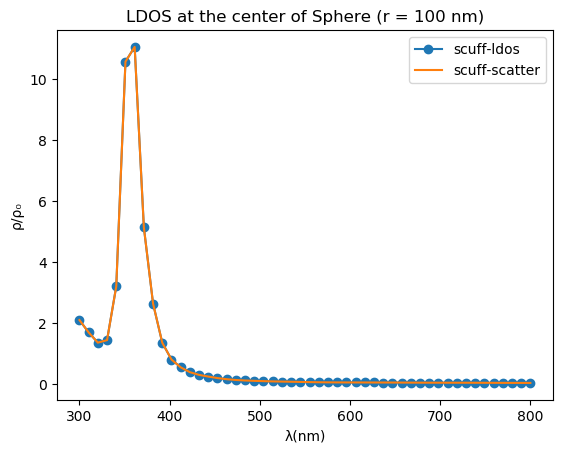
\includegraphics[width=0.45\linewidth]{Sphere100.png}
%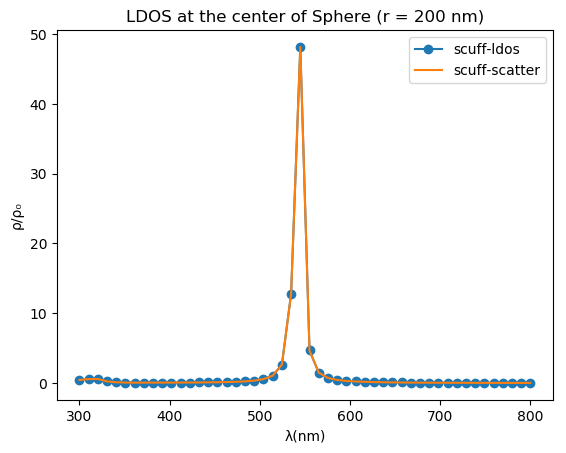
\includegraphics[width=0.45\linewidth]{Sphere200.png}
%%\caption{Caption\label{fig1} }
%\end{figure}

In Owen's thesis, we have that for a shape deformation $\delta x_n(\mathbf{x}^\prime)$, the variation for the object function $F$ is (Eq. (5.28) in Ref. \cite{thesis}). 
\begin{equation}
\delta F = 2Re\int \delta x_n(\mathbf{x}^\prime) [(\epsilon_2 -\epsilon_1) \mathbf{E}_{\parallel}(\mathbf{x}^\prime)\cdot\mathbf{E}^\mathbf{A}_{\parallel}(\mathbf{x}^\prime) + (\frac{1}{\epsilon_1}-\frac{1}{\epsilon_2})\mathbf{D}_{\perp}(\mathbf{x}^\prime)\cdot\mathbf{D}^\mathbf{A}_{\perp}(\mathbf{x}^\prime)]dA
\end{equation}
However, this equation is wrong because it assumed that $\partial F/\partial \mathbf{E}$ is the complex conjugate of $\partial F/\partial \mathbf{\bar{E}}$. In fact,
\begin{equation}
\overline{(\frac{F}{\partial \mathbf{E}})}=\frac{\partial \bar{F}}{\partial\bar{\mathbf{E}}} \neq \frac{\partial F}{\partial \mathbf{\bar{E}}}
\end{equation}

Therefore, the right variation for the object function should be
\begin{equation}
\delta F = \int \delta x_n(\mathbf{x}^\prime) [(\epsilon_2 -\epsilon_1) \mathbf{E}_{\parallel}(\mathbf{x}^\prime)\cdot\mathbf{E}^\mathbf{A}_{\parallel}(\mathbf{x}^\prime) + (\frac{1}{\epsilon_1}-\frac{1}{\epsilon_2})\mathbf{D}_{\perp}(\mathbf{x}^\prime)\cdot\mathbf{D}^\mathbf{A}_{\perp}(\mathbf{x}^\prime)]dA + \text{Conjugate Adjoint}.
\end{equation}

Since the electric LDOS $\rho_e$ is the imaginary part of some function, say $\tilde{\rho_e}$. The optimum of $\tilde{\rho_e}$ must also be the optimum of $\rho_e$. So we can first take the object function to be $\tilde{\rho_e}$, for each direction $j$ in Eq. \eqref{rhoe}, the source of the adjoint field is a electric dipole at $\mathbf{x}_0$ with the amplitude 
\begin{equation}
\frac{\partial \tilde{\rho_e}}{\partial \mathbf{E}_{s_j}} = \frac{\epsilon_0}{\pi\omega}\int dx^3\delta(\mathbf{x}-\mathbf{x}_0)\hat{\mathbf{s}_j}
\end{equation}
while the conjugate adjoint field part $\frac{\partial \tilde{\rho_e}}{\partial \mathbf{\bar{E}}_{s_j}} =0$.

This is a also a dipole at $\mathbf{x}=\mathbf{x}_0$ in the $\hat{\mathbf{s}_j}$ direction, so the adjoint field is the same as the original field up to a constant scalar:
\begin{equation}
\mathbf{E}^\mathbf{A}_{s_j}(\mathbf{x}) = \frac{\epsilon_0}{\pi\omega}\mathbf{E}_{sj}
\end{equation}
Therefore, we have the variation for the electric LDOS as
\begin{equation}
\delta \rho_e =  \frac{\epsilon_0}{\pi\omega}Im\sum_j\int \delta x_n(\mathbf{x}^\prime) \{(\epsilon_2 -\epsilon_1) [\mathbf{E}_{s_j\parallel}(\mathbf{x}^\prime)]^2+ (\frac{1}{\epsilon_1}-\frac{1}{\epsilon_2})[\mathbf{D}_{s_j\perp}(\mathbf{x}^\prime)]^2\}dA\label{fderiv}
\end{equation}

In \verb|scuff-scatter|, we can use $\verb|--EPFile|$ to get the electric field of specified points, however, it only applies to points away from the scattering surface. For points on the surface, the obtained data are just garbage. Instead, we can implement the option $\verb|--PSDFile|$ to obtain the effective electric and magnetic surface charge and current. In the $\verb|scuff|$ calculation, the effective electric and magnetic surface charge and current are defined as

\begin{subequations}
\begin{eqnarray}
\sigma &=& \mathbf{n}\cdot\mathbf{D}\\
\mathbf{K} & =& \mathbf{n}\times\mathbf{H}\\
\eta &=& \mathbf{n}\cdot\mathbf{B}\\
\mathbf{N} & =& \mathbf{n}\times\mathbf{E}
\end{eqnarray}
\end{subequations}

Therefore, the parallel electrical field and perpendicular displacement can be computed as
\begin{subequations}
\begin{eqnarray}
\mathbf{E}_\parallel &=& \mathbf{N}\\
\mathbf{D}_\perp &=& \sigma\mathbf{n}
\end{eqnarray}
\end{subequations}

%The gradient direction is then 
%\begin{equation}
%\frac{\partial \rho_e}{\partial x_n(\mathbf{x}^\prime)}=\frac{2\epsilon_0}{\pi\omega}Im\sum_j [(\epsilon_2 -\epsilon_1) |\mathbf{E}_{j\parallel}(\mathbf{x}^\prime)|^2 + (\frac{1}{\epsilon_1}-\frac{1}{\epsilon_2})|\mathbf{D}_{j\perp}(\mathbf{x}^\prime)|^2
%\end{equation}
%for every $\mathbf{x}^\prime$ on the surface $A$.

After the surface fields are obtained, we can first verify this adjoint method on a void sphere case. For a void sphere, the electromagnetic surface modes satisfy:
\begin{equation}
\epsilon_m (E) H_l(k_ma)[k_daJ_l(k_da)]^\prime = \epsilon_d J_l(k_da)[k_maH_l(k_ma)]^\prime\label{res}
\end{equation}
where $a$ corresponds to the void radius, $l$ is the (integer) index denoting the angular momentum, $k_m=\sqrt{\epsilon_m}k_0$ and $k_d = \sqrt{\epsilon_d}k_0$ are wave vectors in metal and void. $J_l$ and $H_l$ are spherical Bessel and Hankel functions of the first kind\cite{ESM1,ESM2}. 

By solving Eq. \eqref{res}, we can quickly get some resonant parameters and use it as the initial guess for the general shape optimization purpose. %We did a some verifications on the case of void sphere LDOS.

We use the boost library to create spherical harmonic basis functions. 

\begin{equation}
Y_l^m(\theta,\phi) =\left\{\begin{array}{ll}
\sqrt{\frac{2n+1}{4\pi}\frac{(n-m)!}{(n+m)!}}P_l^m(\cos\theta)\cos(m\phi),&m\leq0\\
\sqrt{\frac{2n+1}{4\pi}\frac{(n-m)!}{(n+m)!}}P_l^m(\cos\theta)\sin(m\phi),&m>0\\\end{array}\right.
\end{equation}

The basis function set contains various combinations of $(l,m)$, we number them by $n=l(l+1)+m+1$, then an arbitrary shape function $x(\theta,\phi)$ can be expressed as 
\begin{equation}
x(\theta,\phi) = c_0 + |\sum_{n=1}^N c_nY_n(\theta,\phi)|^2\label{sh}
\end{equation}
where $c_0=d_{min}$ is the minimum distance and $c_n$ is the expansion coefficients and the parameters that we need to optimize.

In numerical evaluation, we do the surface integral by summing up all panels with each panel $\delta A_p(\theta,\phi)$. Inserting Eq. \eqref{sh} to Eq. \eqref{fderiv} we get

\begin{equation}
\delta \rho_e =  \frac{2\epsilon_0}{\pi\omega}Im\sum_{j,n,p} \delta c_n\sqrt{x-c_0}Y_n(\theta,\phi) \{(\epsilon_2 -\epsilon_1) [\mathbf{E}_{s_j\parallel}(\mathbf{x}^\prime)]^2+ (\frac{1}{\epsilon_1}-\frac{1}{\epsilon_2})[\mathbf{D}_{s_j\perp}(\mathbf{x}^\prime)]^2\}\delta A_p(\theta,\phi).\label{sdelta}
\end{equation}

Since $(\theta,\phi)$ is determined by $\mathbf{x}^\prime$, the derivate to one coefficient $c_n$ is then
\begin{equation}
\frac{\partial \rho_e}{\partial c_n} =  \frac{2\epsilon_0}{\pi\omega}Im\sum_{j,p}\sqrt{x-c_0}Y_n(\mathbf{x}^\prime) \{(\epsilon_2 -\epsilon_1) [\mathbf{E}_{s_j\parallel}(\mathbf{x}^\prime)]^2+ (\frac{1}{\epsilon_1}-\frac{1}{\epsilon_2})[\mathbf{D}_{s_j\perp}(\mathbf{x}^\prime)]^2\}\delta A_p(\mathbf{x}^\prime).\label{sderiv}
\end{equation}
%\begin{figure}[H]
%\centering
%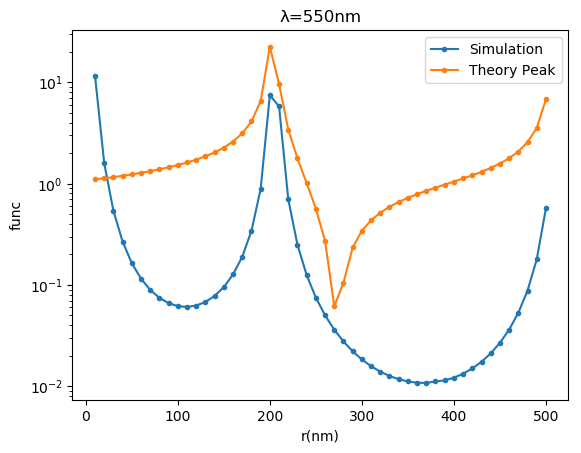
\includegraphics[width=0.45\linewidth]{SV550.png}
%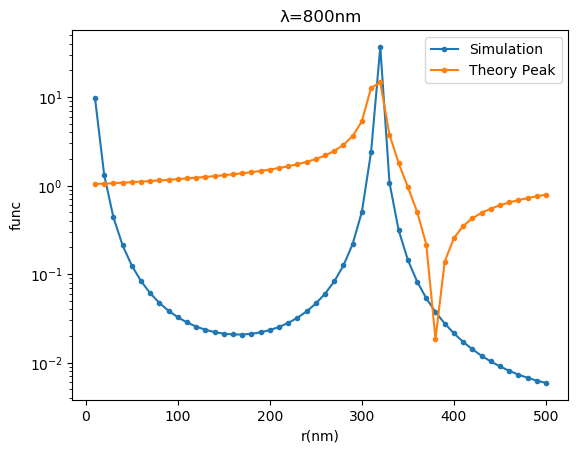
\includegraphics[width=0.45\linewidth]{SV800.png}
%%\caption{Caption\label{fig1} }
%\end{figure}
%\begin{figure}[H]
%\centering
%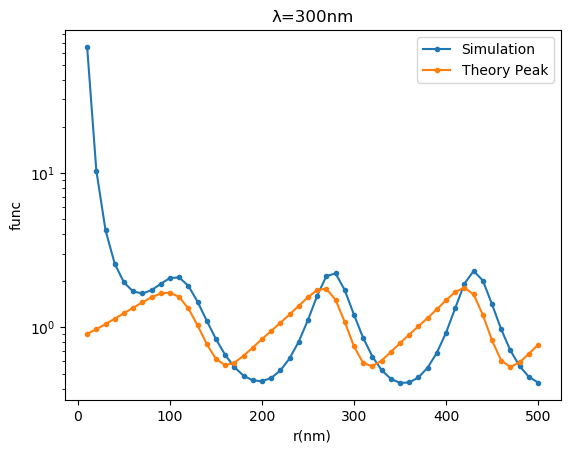
\includegraphics[width=0.45\linewidth]{SV300.png}
%\end{figure}
%At $\lambda = 550$ nm, the resonance is around $r=200$ nm. We do a sweep around $r=200$ nm and check the LDOS as well as the derivative which is obtained from Eq. \eqref{fderiv}. Results are shown below.
%\begin{figure}[H]
%\centering
%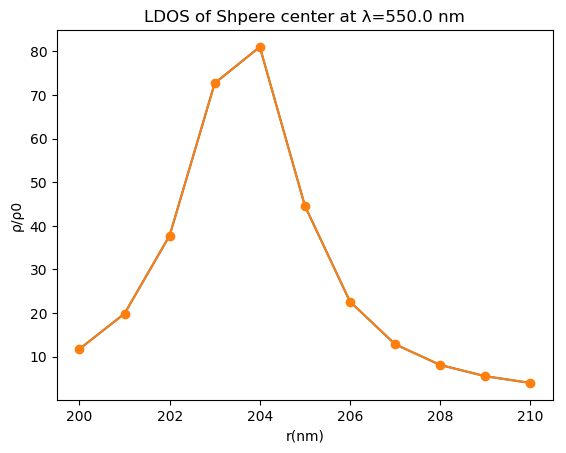
\includegraphics[width=0.45\linewidth]{lambda550_l.png}
%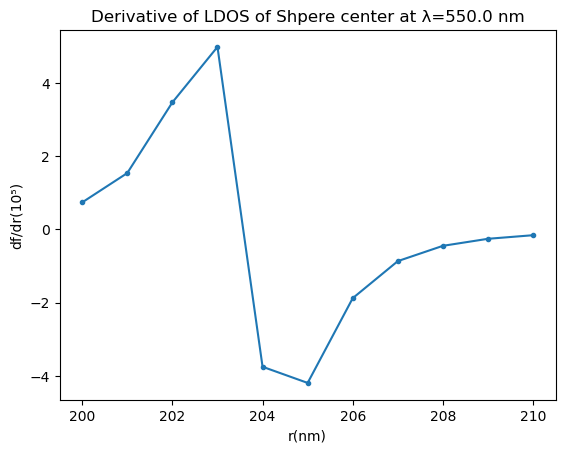
\includegraphics[width=0.45\linewidth]{lambda550_d.png}
%%\caption{Caption\label{fig1} }
%\end{figure}
%
%Similarly, we can do it at $\lambda=800$ nm and 300 nm. 
%\begin{figure}[H]
%\centering
%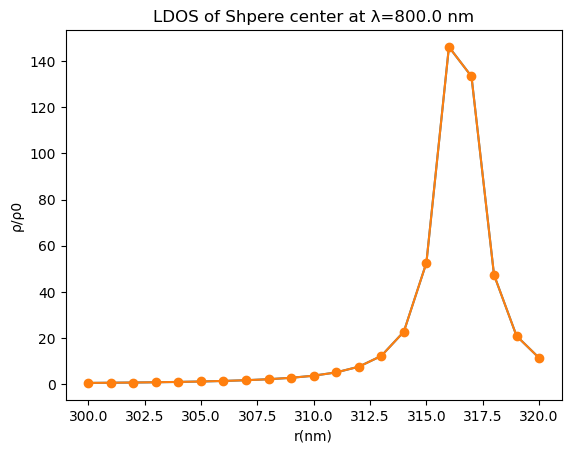
\includegraphics[width=0.45\linewidth]{lambda800_l.png}
%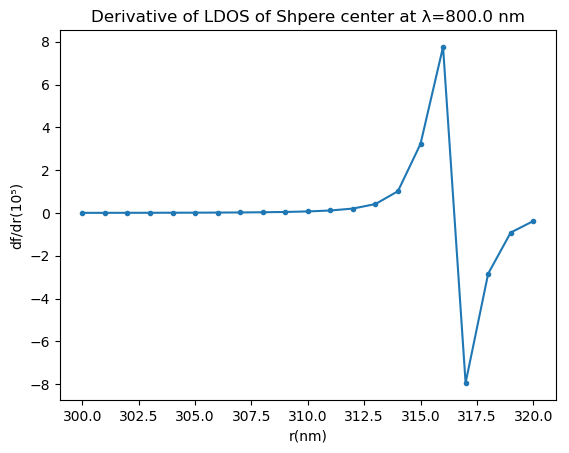
\includegraphics[width=0.45\linewidth]{lambda800_d.png}
%%\caption{Caption\label{fig1} }
%\end{figure}
%
%\begin{figure}[H]
%\centering
%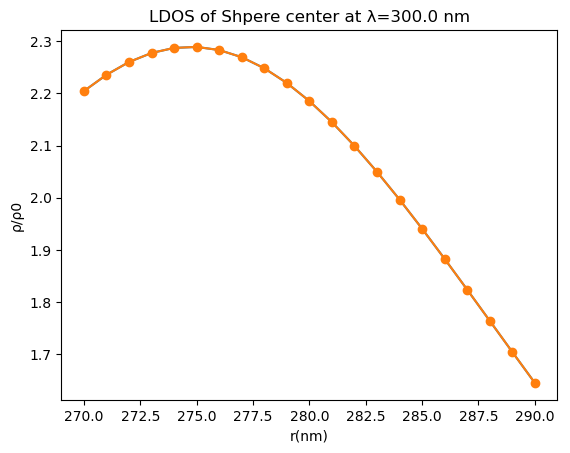
\includegraphics[width=0.45\linewidth]{lambda300_l.png}
%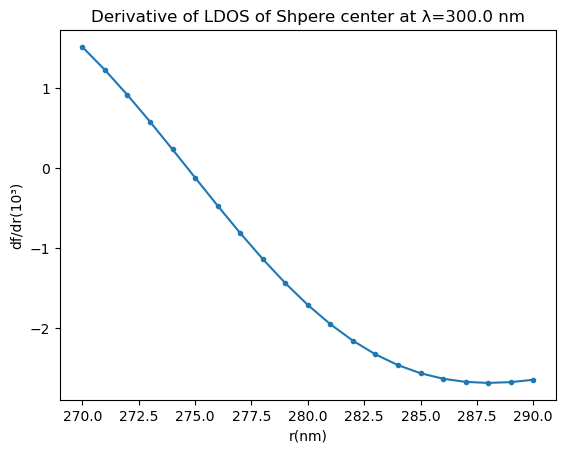
\includegraphics[width=0.45\linewidth]{lambda300_d.png}
%%\caption{Caption\label{fig1} }
%\end{figure}
%To check the validity of the result. We refine our mesh at $\lambda=550$ nm and $r$= 203.5 nm. The results are shown below
%\begin{table}[H]
%\centering
%\begin{tabular}{ccc}
%\hline
%Mesh Size & Number of panels & Derivative \\
%\hline
%1 & 530 & 459650\\
%2  & 1680 & 139513\\
%3 & 3642 & -152891\\
%4 & 6196  & -252036\\
%5 & 10090 & -299709\\
%\hline
%\end{tabular}
%\end{table}
%
%We can see that the maximum is too steep, so the derivative is becoming larger and larger when it approaches the peak. And the result becomes very sensitive to mesh size as it approaches the peak. 

%%%%%%%%%%%%%%%%%%%%%%%%%%%%%Format%%%%%%%%%%%%%%%%%%%%%

%\begin{figure}[H]
%\centering
%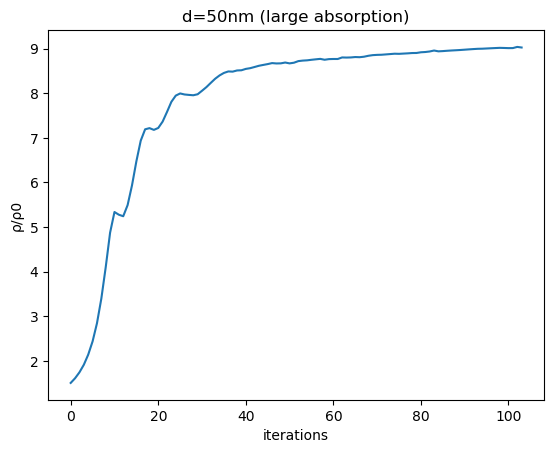
\includegraphics[width=0.9\linewidth]{fig1.png}
%\caption{Caption\label{fig1} }
%\end{figure}
%
%\begin{eqnarray}
%equation array
%\end{eqnarray}
%
\begin{thebibliography}{10}
%\beamertemplatearticlebibitems
%\footnotesize
\bibitem{main}{O. D. Miller, A. G. Polimeridis, M. T. H.Reid, C. W.Hsu, B. G. DeLacy, J. D. Joannopoulos, M. Soljacic, and S. G. Johnson, ``Fundamental limits to optical response in absorptive systems," Opt. Express \textbf{24}, 3329-3364  (2016).} 
\bibitem{halfldos}{ K. Joulain, R. Carminati, J.-P. Mulet, and J.-J. Greffet, ``Definition and measurement of the local density of electromagnetic states close to an interface," Phys. Rev. B \textbf{68}, 245405 (2003).}
\bibitem{thesis}{O. D. Miller, ``Photonic Design: From Fundamental Solar Cell Physics to Computational Inverse Design," PhD Thesis in University of California, Berkeley (2012).}
\bibitem{ESM1}{ M. E. Abdelsalam S. Cintra, S. Mahajan, A. E. Russell, and P. N. Bartlett, ``Localized and delocalized plasmons in metallic nanovoids" Phys. Rev. B \textbf{74}, 245415 (2006).}
\bibitem{ESM2}{ A. D. Boardman, \emph{Electromagnetic Surface Modes}, Wiley-Interscience, 1982}
\end{thebibliography}

\end{document}

